\problemname{Slikhalskæde}
Ane vil dele en slikhalskæde med Bo.
Halskæden består af to slags slik med hhv. blåbær- og vaniljesmag.
For at det skal være retfærdigt, vil Ane dele halskæden i to dele med lige mange stykker slik i hver.
Men Ane synes meget bedre om blåbærsmag end om vanilje, og hun vil derfor have så meget blåbærslik i sin halvdel som muligt.

Hvor mange stykker blåbærslik kan Ane maksimalt få i sin halvdel, hvis hun klipper halskæden over optimalt?

\section*{Indlæsning}
Indlæsningen er en linje bestående af en tekststreng som beskriver halskæden.
Strengen består af bogstaverne \texttt{B} (for »blåbær«) og \texttt{V} (for »vanilje«), dens totale antal bogstaver er et lige tal.

\section*{Udskrift}
Udskriv en linje med et enkelt heltal, det maksimale antal stykker blåbærslik, som Ane kan opnå i sin halvdel af halskæden.

\section*{Pointgivning}

Din løsning køres på en række testfaldsgrupper.
For at få point for en gruppe skal du klare samtlige testfald i gruppen.

\noindent
\begin{tabular}{| l | l | l |}
\hline
Gruppe & Point & Begrænsninger \\ \hline
$1$   & $20$       & Halskæden ser ud som på \href{https://www.progolymp.se/2020/affisch.pdf}{plakaten} \\ \hline
$2$   & $40$       & Halskæden består af højst $1\,000$ stykker slik\\ \hline
$3$   & $40$       & Halskæden består af højst $1\,000\,000$ stykker slik \\ \hline
\end{tabular}

\section*{Forklaring af eksempel 1}
BBVVBVVVBB har længde 10, så Ane skal dele halskæden i to dele med 5 stykker slik i hver.
De mulige dele er BBVVB, BVVBV, VVBVV, VBVVV, BVVVB, VVVBB, VVBBB, VBBBB, BBBBV, BBBVV.
Hun får mest blåbærslik ved at vælge VBBBB eller BBBBV, som hver har $4$ stykker med blåbærsmag.

\begin{figure}[h]
	\centering
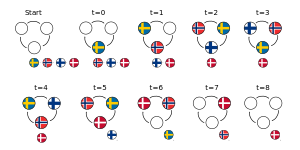
\includegraphics[width=0.5\textwidth]{sample1}
\caption{Et af to optimale løsninger til eksempel 1}
\end{figure}
